% Editable reconstruction; interpretation recorded in root.json.
% Shared standalone design for the editable figure reconstructions.
\documentclass[tikz,border=5pt,10pt]{standalone}
\usepackage[T1]{fontenc}
\usepackage[utf8]{inputenc}
\usepackage{newpxtext,newpxmath}
\usepackage[scaled=.94]{sourcesanspro}
\usepackage{pgfplots}
\pgfplotsset{compat=1.18}
\usetikzlibrary{arrows.meta,calc,positioning,decorations.pathreplacing,
  decorations.markings,patterns,matrix,shapes.geometric,fit,backgrounds,
  intersections,angles,quotes}
\definecolor{ink}{HTML}{203746}
\definecolor{accent}{HTML}{146C78}
\definecolor{muted}{HTML}{667780}
\definecolor{signalred}{HTML}{B94B44}
\color{ink}
\tikzset{>=Latex,line width=.8pt,
  every node/.style={font=\small},
  axis/.style={->,draw=muted,line width=.5pt},
  guide/.style={draw=muted,dashed,line width=.45pt},
  curve/.style={draw=accent,line width=1pt},
  marker/.style={circle,fill=accent,inner sep=1.5pt},
  labelbox/.style={fill=white,inner sep=2pt}}

\begin{document}

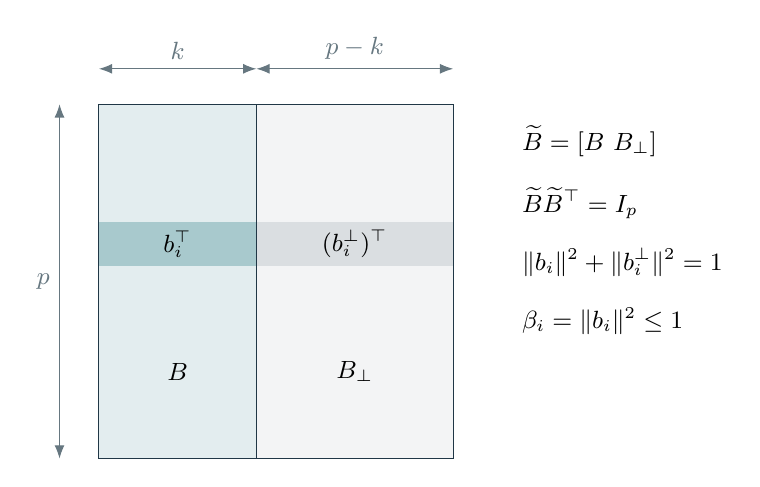
\begin{tikzpicture}
\fill[accent!12] (0,0) rectangle(2,4.5);
\fill[muted!8] (2,0) rectangle(4.5,4.5);
\fill[accent!37] (0,2.45) rectangle(2,3.0);
\fill[muted!24] (2,2.45) rectangle(4.5,3.0);
\draw[ink] (0,0) rectangle(4.5,4.5);\draw[ink] (2,0)--(2,4.5);
\node at (1,2.725) {$b_i^\top$};\node at (3.25,2.725) {$(b_i^\perp)^\top$};
\node at (1,1.1) {$B$};\node at (3.25,1.1) {$B_\perp$};
\draw[<->,muted] (0,4.95)--(2,4.95) node[midway,above] {$k$};
\draw[<->,muted] (2,4.95)--(4.5,4.95) node[midway,above] {$p-k$};
\draw[<->,muted] (-.5,0)--(-.5,4.5) node[midway,left] {$p$};
\node[anchor=west,align=left] at (5.25,2.9) {$\widetilde B=[B\ B_\perp]$\\[10pt]$\widetilde B\widetilde B^\top=I_p$\\[10pt]$\|b_i\|^2+\|b_i^\perp\|^2=1$\\[10pt]$\beta_i=\|b_i\|^2\leq1$};
\end{tikzpicture}
\end{document}
